\section{Introduction}
\label{sec:chapter4_intro}

This chapter presents the development, training, and evaluation of a predictive model aimed at forecasting the outcomes of football matches. The primary objective is to construct a robust model that can accurately predict match results, thereby optimizing gains in sports betting \cite{BaioBlangiardo2010} \cite{DixonColes1997}. The significance of predictive modeling in the context of sports betting lies in its potential to provide bettors with a strategic advantage by identifying value bets and minimizing risks.

\section{Performance Metrics and Selection Criteria}
\label{sec:performance_metrics}

Evaluating the performance of a predictive model in a multi-class classification setting, especially with imbalanced classes, requires a comprehensive set of metrics. This section delineates both classic and advanced metrics employed in this study, incorporating mathematical formulations and addressing class imbalance. Given the three-class problem—home win, draw, and away win—with home wins constituting 47\% of the data, it is crucial to select metrics that provide a nuanced understanding of model performance across all classes.

\subsection{Metrics}
\label{subsec:classic_metrics}

A list of all the metrics considered with their used definition can  be found in Appendix \ref{appendix:predictive_model_metrics}.

\subsection{Selection Criteria}
\label{subsec:selection_criteria}

Accurate evaluation of the predictive model requires appropriate performance metrics, particularly in a multi-class classification context with class imbalance. The primary goal of this study is to ensure that the predicted probabilities of football match outcomes (home win, draw, away win) closely align with the true probabilities, emphasizing well-calibrated probability estimates.

Given the class distribution—47\% home wins, 26\% draws, and 25\% away wins—we have selected the \textbf{Mean Squared Error (MSE)} as the primary metric for assessing calibration. MSE directly measures the average squared difference between predicted probabilities and actual outcomes, making it suitable for evaluating how well the model's probabilities reflect the true frequencies.

In addition to MSE, we will consider the following metrics to provide a comprehensive evaluation:

\begin{itemize}
    \item \textbf{Log Loss}: To assess the quality of the predicted probability distributions by penalizing incorrect and overconfident predictions, thus encouraging well-calibrated estimates.
    \item \textbf{Classwise Expected Calibration Error (ECE)}: To evaluate the calibration of predicted probabilities for each class individually, offering insights into how closely these probabilities match the observed outcomes across different categories.
    \item \textbf{Accuracy for Home Win, Draw, and Away Win}: To examine the model's performance on each outcome separately, taking into account the class imbalance.
\end{itemize}

By focusing on MSE for calibration and incorporating Log Loss, Classwise ECE, and class-specific accuracy, we aim to ensure that the model not only produces accurate probability estimates but also maintains reliability across all outcome categories. This concise set of metrics aligns with our objective of accurately predicting football match outcomes while ensuring the predicted probabilities are well-calibrated and trustworthy.

\section{Exploration and Choice of Features}
\label{sec:feature_selection}

Selecting appropriate features is pivotal for building an effective predictive model. This section delineates the various types of features utilized in this study, the methodology employed for feature selection, the engineering of new features to enhance predictive power, and the handling of categorical variables to ensure they are appropriately represented in the model. 

\subsection{Types of Features Utilized}
\label{subsec:types_features}

The feature set comprises a combination of ranking-based, simple statistical, and domain-specific features. Each feature is defined mathematically where applicable and accompanied by an explanation of its relevance and computation.

\subsubsection{Ranking Features}
\label{subsubsec:ranking_features}

Ranking features provide a quantitative measure of team strength based on historical performance. These metrics are crucial as they encapsulate the overall ability and consistency of teams over time. All ranking features detailed formula are described in \ref{appendix:ranking_features}.

\begin{itemize}

\item \textbf{Elo Score}
\label{par:elo_score}

The \textbf{Elo score} \cite{Elo1978} \cite{HvattumArntzen2010} is a rating system originally developed for chess but widely adapted to various sports to rate players or teams. It reflects the relative skill levels of the teams based on game outcomes.

\begin{figure}[H]
    \centering
    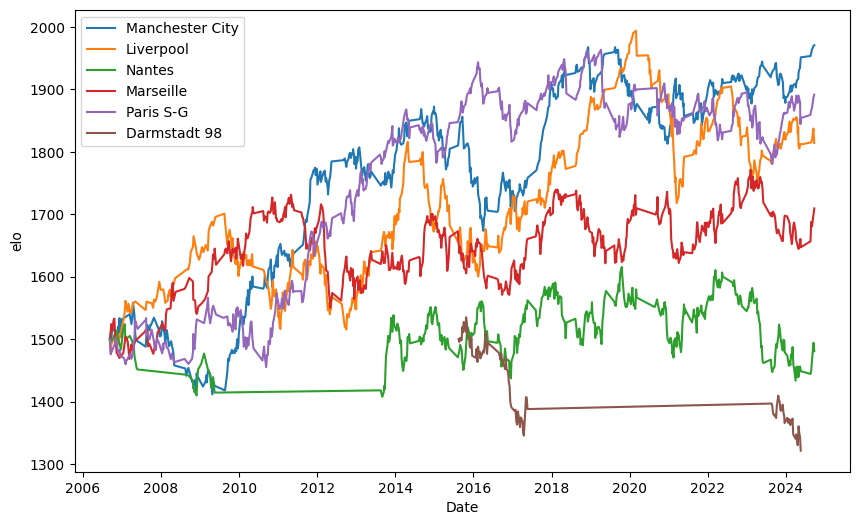
\includegraphics[width=0.8\textwidth, keepaspectratio]{images/elo_score_5_teams_during_time.png}
    \caption{Elo score of 5 football teams evolving during time}
    \label{fig:elo_score_5_teams_during_time}
\end{figure}



\item \textbf{Glicko-2 Score}
\label{par:glicko2_score}

The \textbf{Glicko-2 score} \cite{Glickman1999} is an advanced rating system developed by Mark Glickman, which enhances the Elo rating system by incorporating not only the skill levels of teams or players (R) but also the reliability of these ratings through Rating Deviation (RD) and volatility. This system provides a more dynamic and accurate reflection of performance by accounting for the uncertainty and variability in teams' ratings.


\item \textbf{TrueSkill}
\label{par:trueskill}

The \textbf{TrueSkill} \cite{HerbrichEtAl2007} is a Bayesian ranking system developed by Microsoft, primarily used in gaming but adaptable to sports analytics. It models each team's skill as a Gaussian distribution, updating beliefs about team strengths based on match outcomes.

\end{itemize}

\subsubsection{Simple Statistical Features}


Simple statistical features offer basic quantitative measures of team performance, providing foundational data for the predictive model.


\begin{itemize}
    \item \textbf{Average Goals Scored per Season}: Total goals scored by a team divided by the number of matches played so far.
    
    \item \textbf{Average Goals Conceded per Season}: Total goals conceded by a team divided by the number of matches played so far.
\end{itemize}


\subsubsection{Sofifa Performance Metrics}

SoFIFA provides detailed metrics for both individual players and teams, based on data from the FIFA video game by EA Sports. This document outlines the primary metrics and explains how team ratings are calculated using individual player attributes.

\begin{itemize}

\item \textbf{Player Metrics}
    The primary player metrics on SoFIFA are based on individual attributes that are weighted differently depending on the player's position. Below are the key metrics:
    
    \begin{itemize}
        \item \textbf{Overall Rating (OVR)}: This is the weighted average of various player attributes, with different weights depending on the position. For example, an attacker (\textit{Forward}) will have more emphasis on \textit{Shooting} and \textit{Pace}, while a defender (\textit{Centre Back}) will weigh attributes like \textit{Defending} and \textit{Physicality} more heavily.
        \item \textbf{Pace (PAC)}: Calculated as a combination of the \textit{Acceleration} and \textit{Sprint Speed} attributes.
        \item \textbf{Shooting (SHO)}: Includes \textit{Finishing}, \textit{Shot Power}, \textit{Long Shots}, and \textit{Positioning}.
        \item \textbf{Passing (PAS)}: Comprised of \textit{Vision}, \textit{Short Passing}, and \textit{Long Passing}.
        \item \textbf{Dribbling (DRI)}: Includes \textit{Ball Control}, \textit{Dribbling}, \textit{Agility}, and \textit{Balance}.
        \item \textbf{Defending (DEF)}: Based on \textit{Tackling}, \textit{Marking}, \textit{Interceptions}, and \textit{Defensive Awareness}.
        \item \textbf{Physicality (PHY)}: Includes \textit{Strength}, \textit{Stamina}, and \textit{Aggression}.
        \item \textbf{Potential}: Indicates the maximum possible rating the player can achieve over time.
    \end{itemize}
    
    The formula for the Overall Rating (OVR) is generally unknown, but it can be expressed as a weighted sum of key attributes, depending on the player’s position. A simplified formula for a forward might look like:
    
    \[
    \text{OVR}_{\text{Forward}} = w_1 \cdot \text{PAC} + w_2 \cdot \text{SHO} + w_3 \cdot \text{DRI} + w_4 \cdot \text{PAS}
    \]
    
    where \( w_1, w_2, w_3, w_4 \) are position-specific weights.

\item \textbf{Team Metrics}
    Team metrics on SoFIFA are calculated by aggregating individual player ratings, focusing on key areas like attack, midfield, and defense. The following are the primary team metrics:
    
    \begin{itemize}
        \item \textbf{Overall Team Rating}: A weighted average of the starting 11 players' Overall Ratings, considering the importance of each player's position.
        \item \textbf{Attack Rating}: The average Overall Rating of forwards and attacking midfielders, weighted based on the formation.
        \item \textbf{Midfield Rating}: The average Overall Rating of central and wide midfielders, weighted based on their roles in the formation.
        \item \textbf{Defense Rating}: The average Overall Rating of defenders and goalkeepers.
    \end{itemize}
    
    A simplified version of the team rating could be expressed as:
    
    \[
    \text{Team OVR} = \frac{1}{11} \sum_{i=1}^{11} \text{OVR}_i
    \]
    
    where \( \text{OVR}_i \) represents the Overall Rating of the $i$-th player in the starting lineup.
    
    
    Sofifa metrics are comprehensive team-specific performance indicators sourced from the Sofifa database, widely used in sports analytics and fantasy football contexts.
\end{itemize}

\begin{figure}[H]
    \centering
    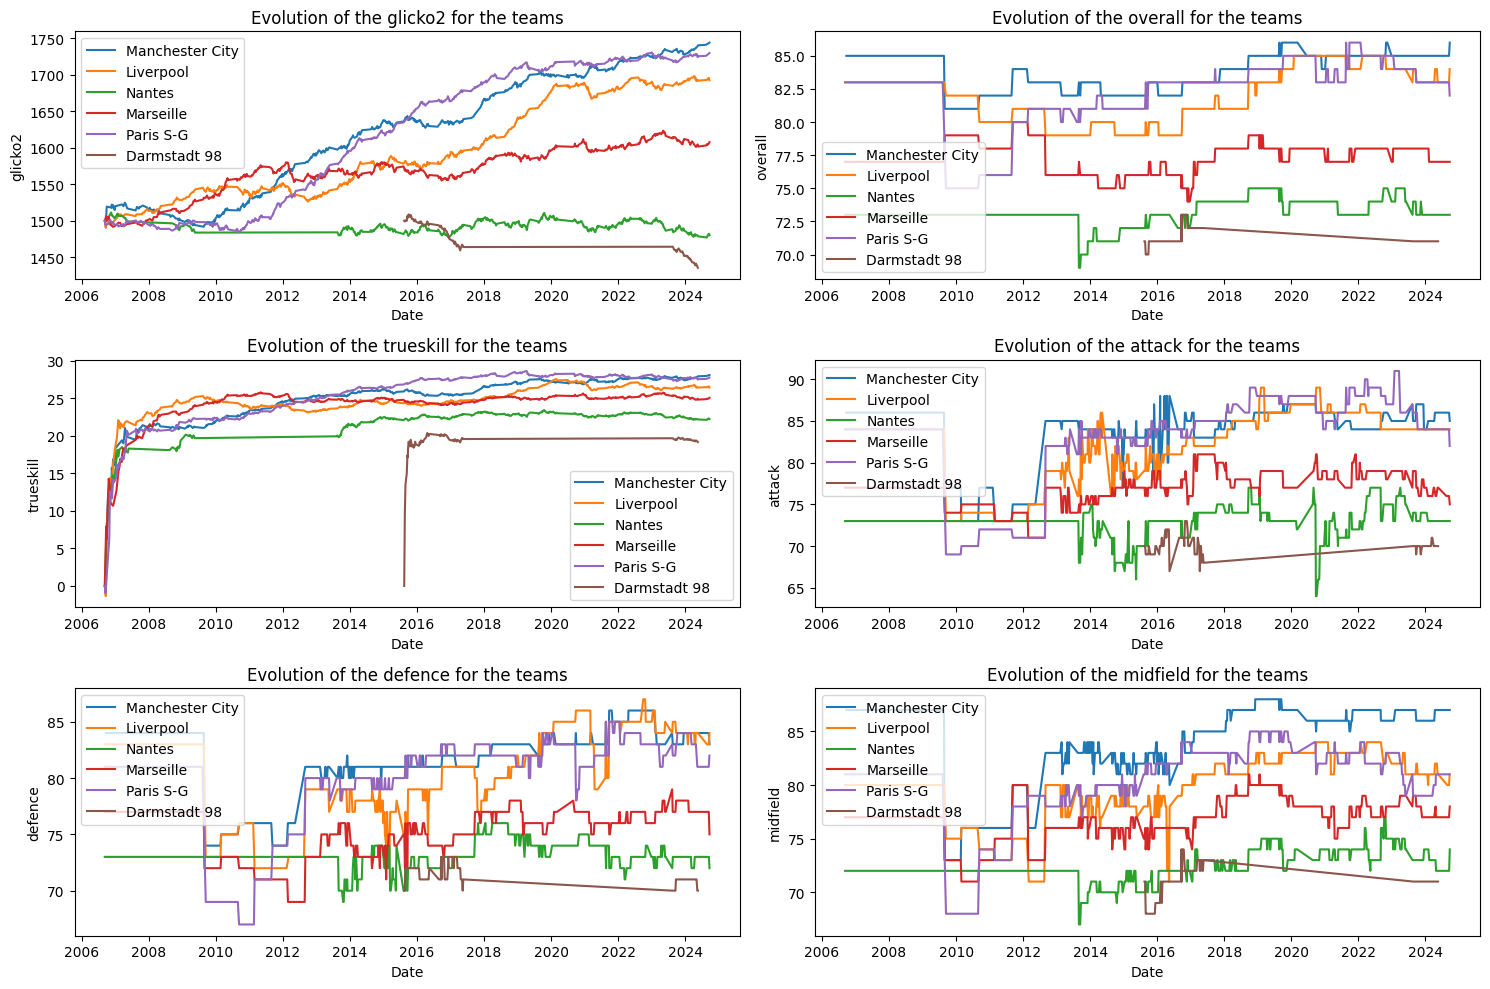
\includegraphics[width=\textwidth, keepaspectratio]{images/scores_5_teams_during_time.png}
    \caption{Different scores of 5 football teams evolving during time}
    \label{fig:scores_5_teams_during_time}
\end{figure}

A detailed description of each of the 90 features used can be found her \ref{appendix:all_feature_descriptions}.

\subsection{Feature Selection Methodology}
\label{subsec:feature_selection_methodology}

Feature selection was performed using a forward selection approach applied to a logistic regression model. This method iteratively adds the most significant features, enhancing predictive performance while maintaining model simplicity.

\subsubsection{Forward Selection with Logistic Regression}
\label{subsubsec:forward_selection_logistic_regression}

\textbf{Procedure}: Starting with no features, at each iteration, the feature that most improves the model's fit is added. The selection criterion is based on the mse (mean squared error).

\textbf{Explanation}: By incorporating features that significantly contribute to the model, forward selection optimizes predictive accuracy and ensures interpretability by excluding irrelevant variables.

\section{Data Preparation}

We trained our model on matches from 2006 to the present, focusing on games from the top 5 European leagues, European championships, and World Cups during this period. The limiting factor in our data came from SoFIFA, which does not provide data prior to 2006, while FBref offers data extending far into the past. We merged the two datasets based on team names and computed the ranking and statistical features described earlier, initializing the metrics at the first entry of a team in a tournament. For categorical features, we applied one-hot encoding. We removed matches with any missing values in the columns, then applied a standard scaler. This left us with 28,850 completed matches and a 90-feature vector for each match to train our model.

\begin{table}[h]
\centering
\begin{tabular}{|l|c|c|}
\hline
\textbf{Metric} & \textbf{Value} \\
\hline
Total matches & 28,850 \\
Matches in Top 5 Leagues & 28,481 \\
Matches in European Championships & 185 \\
Matches in World Cup & 184 \\
Home win ratio & 45.0 \% \\
Draw ratio & 25.4 \% \\
Away win ratio & 29.5 \% \\ 
Average home team goals & 1.54 \\
Average away team goals & 1.19 \\
Average Elo rating & 1558 \\
Number of unique teams & 242 \\
Number of features per match & 90 \\
First match date & 2006-09-09 \\
Last match date & 2024-09-24 \\
\hline
\end{tabular}
\caption{Summary Metrics for the Dataset}
\end{table}


\section{Cross-Validation on Temporal Data}
\label{sec:cross_validation_temporal}

In predictive modeling with football match data, which is inherently temporal, it's essential to use cross-validation techniques that respect the chronological order of observations. Standard cross-validation methods, such as random shuffling or traditional \( k \)-fold cross-validation, are unsuitable because they can lead to data leakage by training models on future data to predict past events.

Traditional cross-validation assumes that data samples are independent and identically distributed (i.i.d.) and that the order of observations does not matter. In temporal data, however, observations are time-dependent, and future events should not influence model training aimed at predicting past events. Using standard methods can result in:

\begin{itemize}
    \item \textbf{Data Leakage}: Incorporating future information into the training set leads to overly optimistic performance estimates.
    \item \textbf{Violation of Temporal Order}: Disrupting the sequence of events undermines the model's ability to generalize to real-world forecasting scenarios.
\end{itemize}


To address these issues, we employ cross-validation methods designed for temporal data \cite{BergmeirEtAl2018}.

\subsection{Sliding Window Cross-Validation}

This technique involves moving a fixed-size window across the data timeline. In each iteration, the model is trained on a training window and tested on the immediately following testing window.

\begin{itemize}
    \item Choose a training window size \( W_{\text{train}} \) and a testing window size \( W_{\text{test}} \).
    \item For each iteration:
    \begin{itemize}
        \item Train the model on data from time \( t \) to \( t + W_{\text{train}} - 1 \).
        \item Test the model on data from \( t + W_{\text{train}} \) to \( t + W_{\text{train}} + W_{\text{test}} - 1 \).
        \item Slide the window forward by \( W_{\text{test}} \) units.
    \end{itemize}
\end{itemize}

\subsection{Expanding Window Cross-Validation}

Also known as growing window, this method expands the training set with each iteration by including more historical data.

\begin{itemize}
    \item Start with an initial training window of size \( W_{\text{initial}} \).
    \item For each iteration:
    \begin{itemize}
        \item Train the model on data from time \( t \) to \( t + W_{\text{train}} - 1 \), where \( W_{\text{train}} \) increases with each iteration.
        \item Test on the subsequent data from \( t + W_{\text{train}} \) to \( t + W_{\text{train}} + W_{\text{test}} - 1 \).
        \item Expand the training window to include the latest testing window.
    \end{itemize}
\end{itemize}

\begin{figure}[H]
    \centering
    \begin{minipage}{0.45\textwidth}
        \centering
        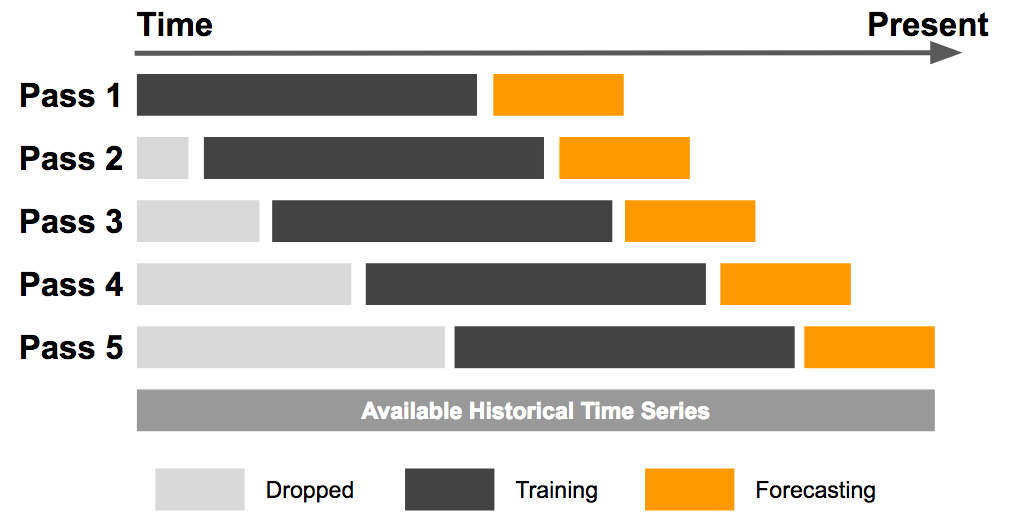
\includegraphics[width=\textwidth, keepaspectratio]{images/FixedWindow.png}
        \caption{Sliding window graphic}
        \label{fig:sliding_window}
    \end{minipage}\hfill
    \begin{minipage}{0.45\textwidth}
        \centering
        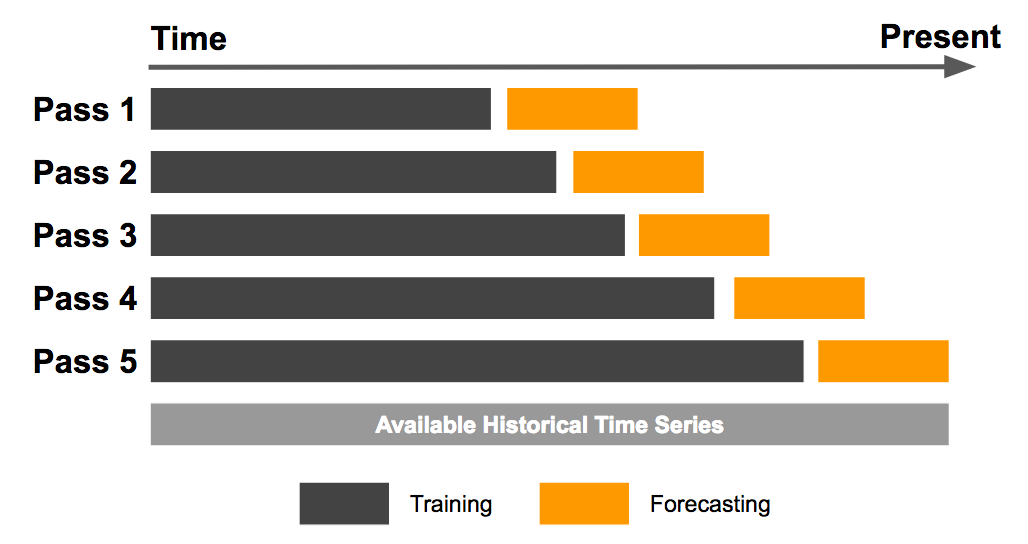
\includegraphics[width=\textwidth, keepaspectratio]{images/ExpandingWindow.png}
        \caption{Expanding window graphic}
        \label{fig:expanding_window}
    \end{minipage}
\end{figure}


The results presented below were obtained using an expanding window technique with 5 folds and a test set ratio of 0.2. Notably, the results were very similar when applying the sliding window method.


\section{Choice and Justification of the Prediction Model}
\label{sec:model_choice}

In this section, we present the results of the feature selection and model selection processes \cite{GuyonElisseeff2003} \cite{ChandrashekarSahin2014}, followed by interpretations of the selected model's performance. Feature selection was conducted using forward selection, and multiple classification models were evaluated to determine the most suitable model for predicting football match outcomes.

\subsection{Feature Selection Using Forward Selection}
\label{subsec:feature_selection}

Feature selection was performed using forward selection with logistic regression, iteratively adding the most significant feature at each step based on mean squared error (MSE) improvement, using an expanding window validation with 5 splits and a test size of 20\% of the training data.

\begin{table}[H]
    \centering
    \caption{Feature Selection Process Summary}
    \label{tab:feature_selection_summary}
    \begin{tabular}{lc}
        \toprule
        \textbf{Method} & \textbf{Details} \\
        \midrule
        Feature Selection & Forward Selection \\
        Model Used & Logistic Regression \\
        Validation Method & Expanding Window (5 splits) \\
        Performance Metric & Mean Squared Error (MSE) \\
        Test Size & 20\% of training data \\
        \bottomrule
    \end{tabular}
\end{table}


We selected 35 features, which corresponding to the features resulting in the lowest MSE, using this feature selection strategy.

\begin{table}[H]
    \centering
    \caption{Feature Selection with Corresponding MSE and their adding number}
    \label{tab:feature_mse}
    \begin{tabular}{|c|l|c|c|l|c|}
        \hline
        \textbf{Order} & \textbf{Feature Added} & \textbf{MSE} & \textbf{Order} & \textbf{Feature Added} & \textbf{MSE} \\
        \hline
        1  & Elo Away & 0.20613 & 19 & Home Passing Risky & 0.19438 \\
        2  & Elo Home & 0.19661 & 20 & Away Positioning Org. & 0.19436 \\
        3  & Glicko Vol Away & 0.19619 & 21 & Away Defense Pressure Med & 0.19435 \\
        4  & Away Overall & 0.19594 & 22 & Away Domestic Prestige & 0.19434 \\
        5  & Home Overall & 0.19540 & 23 & Away Shooting Lots & 0.19433 \\
        6  & Away Build Speed Slow & 0.19518 & 24 & Home Defense Line Offside & 0.19432 \\
        7  & Away Avg Age & 0.19501 & 25 & Away Team Width & 0.19431 \\
        8  & Home League INT & 0.19487 & 26 & Home Defense Pressure Med & 0.19431 \\
        9  & Home Avg Goals & 0.19476 & 27 & Home Build Speed Slow & 0.19430 \\
        10 & Home Positioning Org. & 0.19467 & 28 & Away Defense Aggression & 0.19430 \\
        11 & Home Build Speed Fast & 0.19461 & 29 & TrueSkill Home & 0.19430 \\
        12 & Away Defense Pressure High & 0.19457 & 30 & Away Build Positioning Org. & 0.19430 \\
        13 & Away Defense Offside Trap & 0.19453 & 31 & Away Defense & 0.19430 \\
        14 & Home League ITA & 0.19449 & 32 & Home Attack & 0.19427 \\
        15 & Glicko RD Home & 0.19447 & 33 & Home Defense Prestige & 0.19427 \\
        16 & Home Shooting Normal & 0.19444 & 34 & Away Attack & 0.19427 \\
        17 & Away Passing Mixed & 0.19442 & 35 & Away League INT & \textbf{0.19427} \\
        18 & Away Avg Goals & 0.19440 & & \\
        \hline
    \end{tabular}
\end{table}

The table above summarizes the features added during the selection process and their corresponding MSE values, highlighting the importance of each feature as it contributes to minimizing the error. As we can see, features such as Elo ratings and overall team metrics play a significant role \cite{LasekEtAl2013}. Now, let's examine how the number of features impacts the performance metrics more broadly, as shown in the following feature selection graph.

\begin{figure}[H]
    \centering
    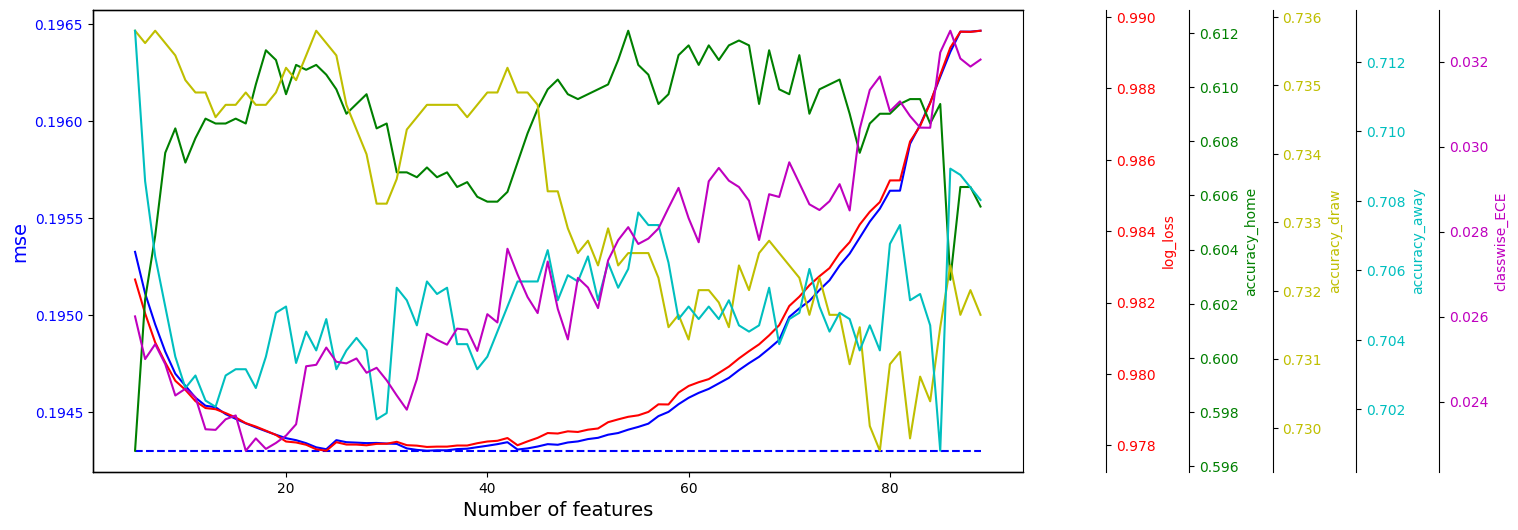
\includegraphics[width=\textwidth, keepaspectratio]{images/feature_selection_metrics_by_nb_of_features.png}
    \caption{Metrics of interrest function of the number of features added}
    \label{fig:feature_selection_metrics_by_nb_of_features}
\end{figure}

This graph shows the performance of various metrics (MSE, log loss, accuracy for home, draw, and away predictions, and classwise ECE) as a function of the number of selected features. The MSE (in blue) decreases as more features are added, stabilizing around the optimal point before increasing again, which suggests that selecting too many features can lead to overfitting. Similarly, log loss follows a similar trend (in red), indicating better model calibration with fewer features. The accuracy metrics (home, draw, away) fluctuate, but accuracy seems to peak at a certain range of features, with performance diminishing as more features are added. Classwise ECE (in pink) decreases and then increases, a little bit before MSE and log loss, indicating better calibration for class predictions with fewer features. Overall, the graph highlights the balance between feature selection and model performance, suggesting that an optimal subset of features yields the best generalization.

\subsection{Model Selection}
\label{subsec:model_selection}

The following table summarizes the performance of various classification models \cite{Bishop2006}, comparing metrics such as mean squared error (MSE), log loss, classwise ECE, and accuracy for home, draw, and away predictions to identify the best-performing model.

\begin{table}[H]
    \centering
    \caption{Model Performance Comparison}
    \label{tab:model_performance}
    \begin{tabular}{|l|c|c|c|c|c|c|}
        \hline
        \textbf{Model} & \textbf{MSE} & \textbf{Log Loss} & \textbf{C. ECE} & \textbf{A. Home} & \textbf{A. Draw} & \textbf{A. Away} \\
        \hline
        Logistic Regression & \textbf{0.195} & \textbf{0.983} & 0.029 & 0.605 & 0.733 & 0.702 \\
        Logistic Regression CV & 0.196 & 0.983 & \textbf{0.028} & 0.602 & \textbf{0.735} & 0.703 \\
        Gradient Boosting Classifier & 0.199 & 1.002 & 0.037 & 0.604 & 0.709 & \textbf{0.706} \\
        Random Forest Classifier & 0.202 & 1.022 & 0.038 & 0.595 & 0.705 & 0.693 \\
        Extra Trees Classifier & 0.204 & 1.026 & 0.043 & 0.597 & 0.683 & 0.686 \\
        AdaBoost Classifier & 0.221 & 1.092 & 0.069 & 0.599 & 0.721 & 0.695 \\
        Bagging Classifier & 0.224 & 2.471 & 0.093 & 0.602 & 0.646 & 0.661 \\
        MLP Classifier & 0.224 & 1.187 & 0.108 & 0.585 & 0.665 & 0.684 \\
        K Neighbors Classifier & 0.238 & 5.404 & 0.096 & 0.599 & 0.643 & 0.631 \\
        Gaussian NB & 0.332 & 7.570 & 0.302 & \textbf{0.615} & 0.584 & 0.625 \\
        Quadratic Discriminant Analysis & 0.353 & 10.831 & 0.316 & 0.582 & 0.561 & 0.613 \\
        Decision Tree Classifier & 0.390 & 20.219 & 0.195 & 0.578 & 0.614 & 0.638 \\
        Extra Tree Classifier & 0.399 & 20.686 & 0.200 & 0.559 & 0.615 & 0.628 \\
        \hline
    \end{tabular}
\end{table}


\subsection{Interpretation of Results}
\label{subsec:interpretation}

The selection of the logistic regression model allows for straightforward interpretation of feature effects on the predicted probabilities of match outcomes.

\subsubsection{Feature Importance}

Feature importance was assessed based on the magnitude of the coefficients in the logistic regression model. Below sits the feature importance of the Home win class. Draw and Away win classes analysis can be found in \ref{appendix:feature_importance}.


\begin{figure}[H]
    \centering
    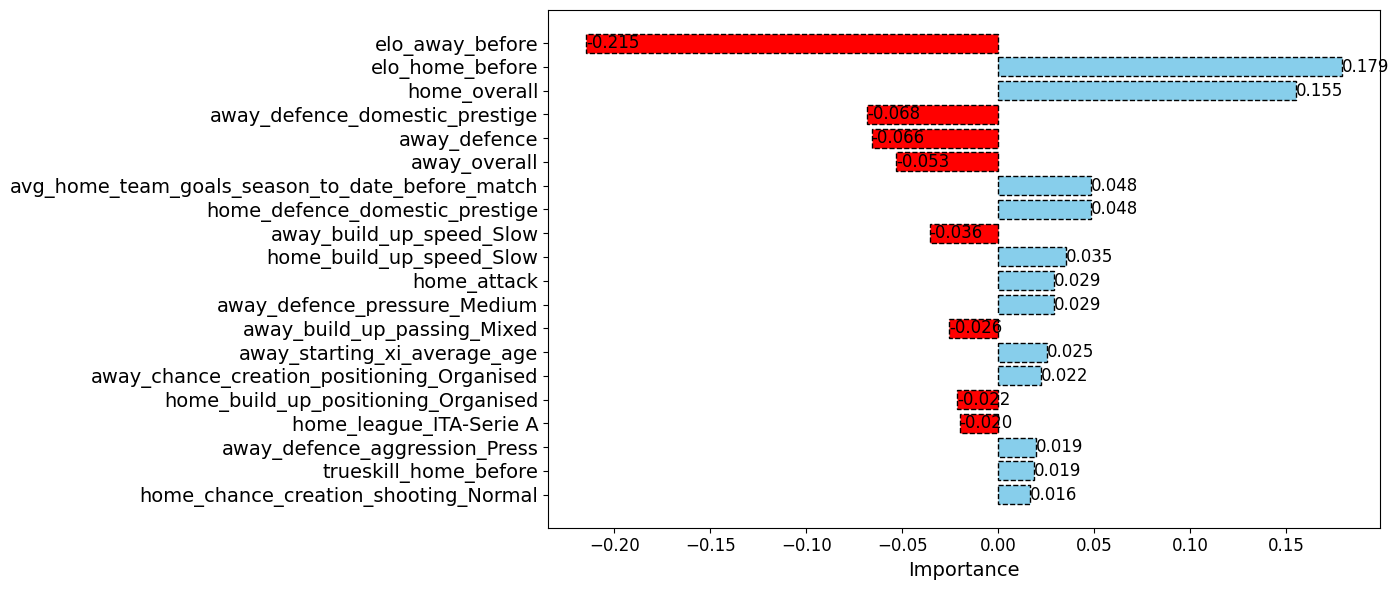
\includegraphics[width=\textwidth, keepaspectratio]{images/top20_coeff_importance_lr_selected_features_home.png}
    \caption{Coefficients of the Logistic Regression Model for Home win class}
    \label{fig:feature_coefficients}
\end{figure}

For the home class, the most important features, such as Elo ratings for the away and home teams, suggest that pre-match team strength is the most significant predictor of match outcomes. Both overall team quality and specific defensive attributes, like pressure and aggression, also play a key role. Features related to player average characteristics, such as average age and tactical elements like build-up speed, indicate that team composition and playstyle are also relevant, though their impact is less pronounced. Defensive strategies, particularly pressure and team width, add further predictive value, showing the importance of tactical decisions in determining match results. The feature importance analysis graphs for draw and away class can be found in the annex section.


\subsubsection{Why Logistic Regression Outperforms Other Models}

Logistic regression may outperform other models due to its simplicity and interpretability, especially when feature selection is based on it. By using logistic regression for feature selection, the model is specifically tuned to highlight the most important predictors of the outcome, leading to better generalization. Additionally, logistic regression handles multicollinearity well when regularization is applied, preventing overfitting. The linear relationship between the features and the log-odds of the outcomes makes it easier to capture important patterns in the data, particularly in problems like sports prediction where relationships between variables are often linear. Other models, such as random forests or gradient boosting, may add unnecessary complexity and are more prone to overfitting when features are already well-selected.


\section{Training and Retraining of the Model}
\label{sec:training_retraining}

Figure \ref{fig:mse_retraining} illustrates the Mean Squared Error (MSE) of two models over time, where the blue line represents Model A with no retraining, and the orange line represents Model B, which is retrained daily. Both models are initialy trained from 2006-01-01 up to 2010-01-01 data and are evaluated using a 120-day rolling average.

\begin{figure}[H]
    \centering
    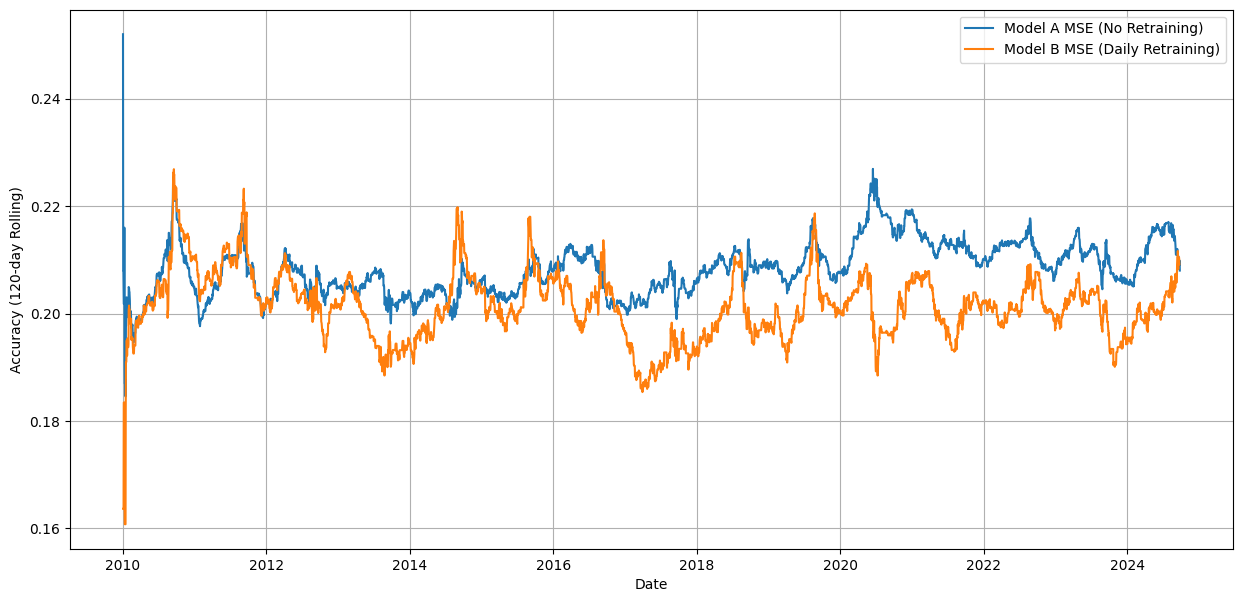
\includegraphics[width=0.8\textwidth, keepaspectratio]{images/model_ratrining_mse_120rd.png}
    \caption{Model MSE rolling average over time}
    \label{fig:mse_retraining}
\end{figure}


From the figure, we observe that Model B, which is frequently retrained, exhibits lower MSE compared to Model A throughout most of the time period. Retraining appears to allow Model B to adapt more effectively to evolving patterns, leading to consistently better performance in terms of accuracy. Moreover, as time goes by, we can observe a mse drift from the not retrained model as well as a slight improvement from the retrained model. \\

There are very few periods where Model A outperforms Model B. It appends especially during phases of sudden changes. Despite these fluctuations, retraining offers a more stable and improved long-term performance. \\

The results highlight the importance of regular retraining for maintaining model accuracy, particularly in dynamic environments where data patterns change over time.

\section{Conclusion}

This chapter presented the development, training, and evaluation of a predictive model for football match outcomes, with a focus on sports betting. Feature selection via forward selection with logistic regression helped identify key predictors, and regular retraining improved model performance over time.\\

However, several limitations remain:

\begin{itemize}
    \item \textbf{Hyperparameters and Features}: Ranking feature hyperparameters were left at default, and additional domain-specific or external data sources could further improve predictions.
    \item \textbf{Feature Selection}: Feature selection was arbitrarily based on logistic regression, and no hyperparameter optimization was performed for any models.
    \item \textbf{Retraining}: The timing and method of retraining (e.g., sliding window) were not explored, potentially missing optimal strategies as well as posing computational challenges that could be optimized.
    \item \textbf{Model Complexity}: Incorporating deep learning models could enhance predictive performance, particularly for capturing complex patterns in the data.
    \item \textbf{Bookmaker Odds Decorrelation}: Adding a metric to assess the decorrelation between model predictions and bookmaker odds could help identify more value bets and further optimize betting strategies.
\end{itemize}
In the next chapter, we address the optimization problem of determining the bankroll share to invest on each outcome, building on the predictions of this model to develop actionable betting strategies.